%iffalse
\let\negmedspace\undefined
\let\negthickspace\undefined
\documentclass[journal,12pt,onecolumn]{IEEEtran}
\usepackage{cite}
\usepackage{amsmath,amssymb,amsfonts,amsthm}
\usepackage{algorithmic}
\usepackage{multicol}
\usepackage{graphicx}
\usepackage{textcomp}
\usepackage{xcolor}
\usepackage{txfonts}
\usepackage{listings}
\usepackage{enumitem}
\usepackage{mathtools}
\usepackage{gensymb}
\usepackage{comment}
\usepackage[breaklinks=true]{hyperref}
\usepackage{tkz-euclide} 
\usepackage{listings}
\usepackage{gvv}                                        
%\def\inputGnumericTable{}                                 
\usepackage[latin1]{inputenc}                                
\usepackage{color}                                            
\usepackage{array}                                            
\usepackage{longtable}                                       
\usepackage{calc}                                             
\usepackage{multirow}                                         
\usepackage{hhline}                                           
\usepackage{ifthen}                                           
\usepackage{lscape}
\usepackage{tabularx}
\usepackage{array}
\usepackage{float}
\newtheorem{theorem}{Theorem}[section]
\newtheorem{problem}{Problem}
\newtheorem{proposition}{Proposition}[section]
\newtheorem{lemma}{Lemma}[section]
\newtheorem{corollary}[theorem]{Corollary}
\newtheorem{example}{Example}[section]
\newtheorem{definition}[problem]{Definition}
\newcommand{\BEQA}{\begin{eqnarray}}
\newcommand{\EEQA}{\end{eqnarray}}
\newcommand{\define}{\stackrel{\triangle}{=}}
\theoremstyle{remark}
\newtheorem{rem}{Remark}

% Marks the beginning of the document
\begin{document}
\bibliographystyle{IEEEtran}
\vspace{3cm}

\title{\textbf{NCERT 6.6.9}}
\author{EE24BTECH11032- John Bobby}
\maketitle
\bigskip
\textbf{Question:}A tank with rectangular base and rectangular sides, open at the top is to be constructed so that its depth is $2$ m and volume is $8$ $m^3$. If building of tank costs  $70$ per sq. meter for the base and  $45$ per square meter for sides. What is the cost of least expensive tank?\\

\textbf{Solution:} Let the length be $x$ and the breadth be $y$\\
\section{Theoretical Approach}
\begin{align}
    \text{Volume}=\brak{2}\brak{x}\brak{y}=8\\
    xy=4\\
    \text{Total Cost}=70\brak{xy}+45\times2\brak{2x+2y}=280+180\brak{x+y}
\end{align}
From equation $\brak{2}$
\begin{align}
    \text{Total Cost}=280+180x+\frac{720}{x}
\end{align}
Differentiating wrt to x on both sides,
\begin{align}
    \frac{dy}{dx}=180-\frac{720}{x^2}
\end{align}
To be a critical point $\frac{dy}{dx}$  must be zero,
\begin{align}
    180-\frac{720}{x^2}=0\\
    x^2=\frac{720}{180}\\
    x=\pm 2\\
\end{align}
$x=2$ as length cant be negative\\
Checking $\frac{d^2y}{dx^2}$ to be positive for minimum
\begin{align}
    \frac{d^2y}{dx^2}=\frac{1440}{x^3}\\
    \frac{d^2y}{dx^2} >0\text{ for }  x=2
\end{align}
Thus $x=2$ is the minimum

\section{Gradient Descent}
\begin{align}
    x_{n+1}=x_n-\alpha f^{\prime}\brak{x_n}\\
     x_{n+1}=x_n-\alpha \brak{180-\frac{720}{{x_n}^2}}
\end{align}
Where $\alpha$ is the learning rate,\\
This iteration will stop until we reach a stable state $\brak{f^{\prime}\brak{x} \approx0}$\\
We get,\\
$x_{min}=2$\\
We can also solve using geometric programming by using the cvpxy module in python. On running the code we get the minimum value of x to be 2.\\
For using quadratic programming we can assume a new variable $y$ as $\frac{1}{x}$, but the constraint will be non-linear but it can be solved as cvxpy supports this structure.
\begin{figure}[h]
\centering
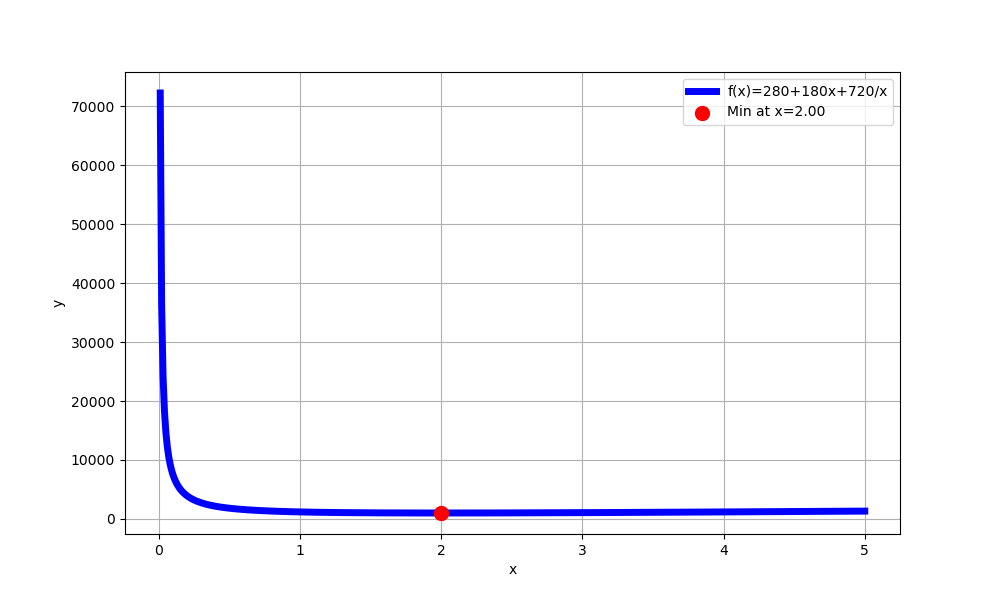
\includegraphics[width=\columnwidth]{figs/Q4.png}
\end{figure}


\end{document}
